
\documentclass{beamer}
\usepackage[utf8]{inputenc}
\usepackage{graphicx}
\usepackage{wrapfig}
\usepackage{xcolor}






\usetheme{Madrid}

\AtBeginSection[]{
	\begin{frame}
		\vfill
		\centering
		\begin{beamercolorbox}[sep=8pt,center,shadow=true,rounded=true]{title}
			\usebeamerfont{title}\insertsectionhead\par%
		\end{beamercolorbox}
		\vfill
	\end{frame}
}

\title{Replication Study: Machine Labor (Angrist, 2022)}
\subtitle {Research Module Econometrics}
\author{Cristian Gutierrez, Marcel Wachter}
\centering
\date{January 14, 2023}
\begin{document}
\maketitle

\begin{frame}
\frametitle{Overview} 

\begin{itemize}
    

\item Research Question
\item Motivation
\item Theory
\item Replication Study
\item XXX
\item XXX
\item Conclusion
\end{itemize}
\end{frame}


\begin{frame}{}

\begin{itemize}

\begin{figure}[htp]
    \centering
    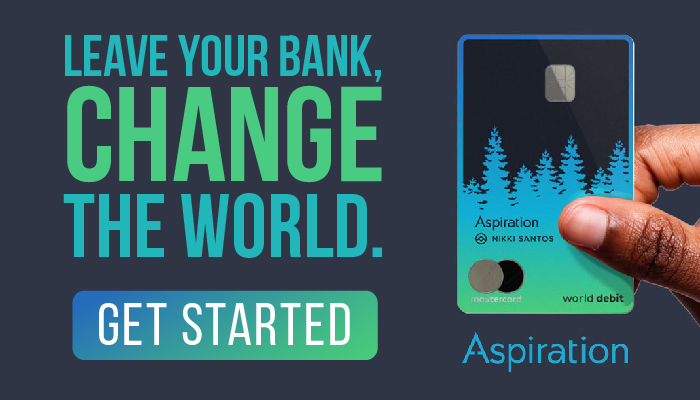
\includegraphics[width=9cm]{cover2.jpg}
    
\end{figure}


 \centering   \textbf{Change text here and remove image. Maybe add a regression table to motivate work}

    


\end{itemize}
\end{frame}

\begin{frame} {Research Question + Main idea of Angrist (2022)}
\begin{itemize}

\item  Angrist (2022) studies utility of machine learning (ML) algorithms for regression-based causal inference using lasso to select control variables for estimates of college characteristics' wage effect.
\item **Add text here**.
\end{itemize}

\end{frame}


\begin{frame}{}

\begin{itemize}

\begin{figure}[htp]
    \centering
    \includegraphics[width=9cm]{Aspiration #4.jpg}
    
\end{figure}
    


\end{itemize}
\end{frame}



\begin{frame}{Main Features}

\flushleft \textbf{ Aspiration offers two main products}
\vspace{4mm}
\begin{itemize}
    \item Cash Management Services 
    \item Investment Funds 
\end{itemize}

\end{frame}

\begin{frame}
\begin{columns}
\column{0.4\textwidth}
 Aspiration cash management services include two different accounts.
 \begin{itemize}
    \item Aspiration (Standard) Account
    \item Aspiration Plus 
\end{itemize}

\column{0.6\textwidth}
\begin{figure}[ht]
\begin{right}
\includegraphics[height=3.2in]{Aspiration # 3.jpg}

\end{right}
\end{figure}
\end{columns}

\end{frame}


\begin{frame}{Aspiration - Cash Back Program}
\begin{columns}
\column{0.4\textwidth}
 
\begin{itemize}
  \centering Instead of earning money for shopping at mostly big retailers, Aspiration \textbf{rewards you} for shopping at places that it identifies as making an \textbf{impact on the world}. 
\end{itemize}

\column{0.6\textwidth}
\begin{figure}[ht]
\begin{right}
\includegraphics[height=2.9in]{5.png}

\end{right}
\end{figure}
\end{columns}

\end{frame}





\begin{frame}{Aspiration - AIM}
\begin{itemize}
  
\item Every company that Aspiration partners with has scored high on what they call the \textbf{“Aspiration Impact Measurement’s People and Planet”} score.
\item They look at things like giving, sustainably, workplace equality and transparency before agreeing to partner with companies in their cash back program. 
\item Currently, Aspiration works with \emph"{TOMs}",\emph{Warby Parker}, \emph{Lola}, \emph{This Saves Lives}, \emph{Blue Apron}, \emph {Burst}, and more.
\end{itemize}
\end{frame}

\begin{frame}{Aspiration -- AIM }
    

  

    \begin{figure}[htp]
    \centering
    \includegraphics[width=6.5cm]{AIM.jpg}
    
\end{figure}



\end{frame}

\begin{frame}{Aspiration - Plant Your Change }
\begin{columns}
\column{0.4\textwidth}
 
\begin{itemize}
    
\item Connect Aspiration's  debit or credit card to "Plant Your Change"
\item Aspiration automatically rounds up every purchase to the nearest dollar and plant a tree with the user's spare change.
\end{itemize}

\column{0.6\textwidth}
\begin{figure}[ht]
\begin{right}
\includegraphics[height=2.9in]{PlantYourChange.png}

\end{right}
\end{figure}
\end{columns}

\end{frame}






\begin{frame}{Aspiration - Investment Funds}
\begin{itemize}
\item The Aspiration Redwood Fund uses a rigorous analysis of companies’ sustainable environmental, workplace, and governance practices to find investments best poised for growth
       
        
\item  Redwood Investment Fund
\begin{itemize}
        \item Pay what is fair
        \item ESG indicators for investment selection
        \item 0.5\% fund operation related expenses
        \end{itemize}
        
        
%\vspace{10mm}
\item  Redwood Individual Retirement Account (IRA)
\begin{itemize}
        \item Same conditions as for Redwood Investment Fund 
        \item Tax benefits according to US law
        \end{itemize}


\end{itemize}
\end{frame}

\begin{frame}{Aspiration - Redwood Investment }
\begin{itemize}




  

    \begin{figure}[htp]
    \centering
    \includegraphics[width=12cm]{Fund.jpg}
    
\end{figure}       
        



\end{itemize}
\end{frame}



\begin{frame}{Potential Challenges of Financial Households}
\begin{itemize}
\item \textbf{Finding the right resource}
\begin{itemize} \item The difficulty of finding the right resource is a prominent factor in the Green Fintech Market. New investors entering the market can easily be overwhelmed by the numerous choices available to them.
\end{itemize}

\item \textbf{ Limited capital}
\begin{itemize}
    \item One of the biggest challenges that new investors face is having limited capital available to invest.
\end{itemize}


\item \textbf{Diversification}
\begin{itemize}
    \item Households generally face a problem of under-diversification of portfolios especially when they are new.
\end{itemize}

    



\end{itemize}
\end{frame}

\begin{frame}{Potential Challenges of Financial Households}
\begin{itemize}
\item \textbf{Lack of Product Awareness}
\begin{itemize} \item  New investors entering the market would be less knowledgeable about sustainable financial products. Investors would have difficulty in determining what actually constitutes as sustainable investment options on entering the market.  
\end{itemize}

\item \textbf{Lack of Trust} 
\begin{itemize}
    \item Households/investor may be less willing to participate in sustainable financial investments due to a lack of trust. Investors would question on the nature of these sustainable investments and whether "they are actually sustainable". 
\end{itemize}
\end{itemize}
\end{frame}


\begin{frame}{Advantages of Aspiration}
\begin{columns}
\column{0.4\textwidth}
 
\begin{itemize}
\item Pay-What-You-Want Investing, Fee-Free Banking 
\item Sustainable Mutual Fund
\item High-Yield Savings Rates
\item Automatic Charitable Contributions
\item Cash Back Program, AIM-score
\end{itemize}

\column{0.5\textwidth}
\begin{figure}[ht]

   

\begin{right}

\includegraphics[height=2.5in]{Impact.PNG}

\end{right}

\end{figure}
\end{columns}

\end{frame}



\begin{frame} {Disadvantages of Aspiration}
\begin{itemize}

\item Interest rate only for Aspiration Plus Account
\item Only available in the United States
\item \$1000 limit on withdrawals
\item Limited Investment Choice
\item No Cash Deposits

              
           
\end{itemize}
    
\end{frame}  
\begin{frame} {Suggestions For Improvement}
    \begin{itemize}
        \item Improving their customer support service by including say "live chat box"
        \item Allowing cash deposits 
        \item More options for mutual funds 
         \item Lottery
        \begin{itemize}
            \item Attributing a lottery number to every tree planted could be a good factor in attracting investors. It would also enable Aspiration to stand out from other green fintechs.
        \end{itemize}     
           
    \end{itemize}
    
    
\end{frame}

\begin{frame} {Conclusions}
\begin{itemize}
\item Aspiration is a good choice if you are a US resident looking for an ethical bank that supports sustainable causes, and are fine with having only simple, limited banking services that are not very competitive compared to what most other neobanks offer.  
\item The fees at Aspiration are arguably the biggest reason to sign up for a new account.
\item  Its investment products should be a supplement to your portfolio, not the entire thing.
\end{itemize}
\end{frame}






















\end{document}
